\documentclass[11pt]{article}
\pagestyle{empty}
\usepackage{amsmath,amssymb,amsfonts,setspace,float,enumerate}
\usepackage{graphicx,mathtools}
\usepackage[margin=1in]{geometry}
\usepackage{hyperref}
\usepackage{xcolor}
\hypersetup{
	colorlinks=true,
    linkbordercolor={1 1 1},
    linkcolor = red
}
\parindent 0px
\pagenumbering{gobble}
\singlespacing

\title{Intelligent Scissors Write Up}
\author{David Ye}
\date{\today}

\begin{document}
\maketitle
\section{Edge Weight Model}
I tested intelligent scissors on sample.png (the blue bird).

\begin{figure}[H]
	\centering
	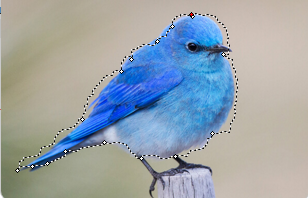
\includegraphics{sample_bad.png}
	\caption{\label{fig:bird_16}Cutting out blue bird using original intelligent scissors with 16 anchors}
\end{figure}

In figure \ref{fig:bird_16}, I cut the blue bird out using 16 anchors. Unfortunately, the cut turned out very rough and did not closely follow the bird's outline. There are small buffers between most of the cuts and the bird's body. Interestingly, the cuts underneath the bird's tail followed the bird very nicely. In figure \ref{fig:bird_5}, I decreased the number of anchors to five, and the cut turned out much worse. There are large buffers between the cut and the bird's back and tail. The scissors also cut through the bird's belly rather than around it.

\begin{figure}[H]
	\centering
	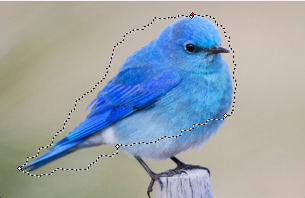
\includegraphics{sample_bad_2.png}
	\caption{\label{fig:bird_5}Cutting out blue bird using original intelligent scissors with five anchors}
\end{figure}

Interestingly, when the Z-crossing score is calculated opposite of the specification (set Z-crossing score to be one when the absolute value of the Laplacian is smaller than its neighbor and zero otherwise), the intelligent scissors improved greatly. In figure \ref{fig:bird_4}, the scissors nicely cut around the bird using just four anchors, which is a huge improvement from before.

\begin{figure}[H]
	\centering
	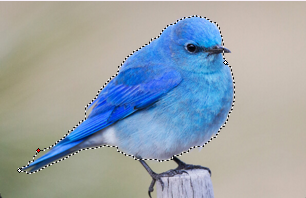
\includegraphics{sample_3anchor.png}
	\caption{\label{fig:bird_4}Cutting out blue bird using modified intelligent scissors with four anchors}
\end{figure}

To find out why the modified scissors worked better than the original, I plotted cost matrices of the bird. Figure \ref{fig:bird_cost_ori} shows the cost matrix using the original Z-crossing score, and figure \ref{fig:bird_cost_mod} shows the cost matrix using the modified Z-crossing score. In both figures, pixels with costs closer to zero appear white and pixels with costs closer to one appear black.

\begin{figure}[H]
	\centering
	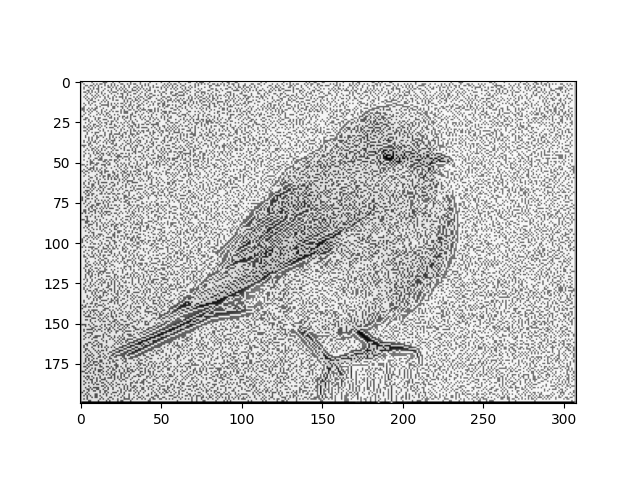
\includegraphics{Cost_Bird_Original.png}
	\caption{\label{fig:bird_cost_ori}Cost matrix of blue bird using original Z-crossing score}
\end{figure}

\begin{figure}[H]
	\centering
	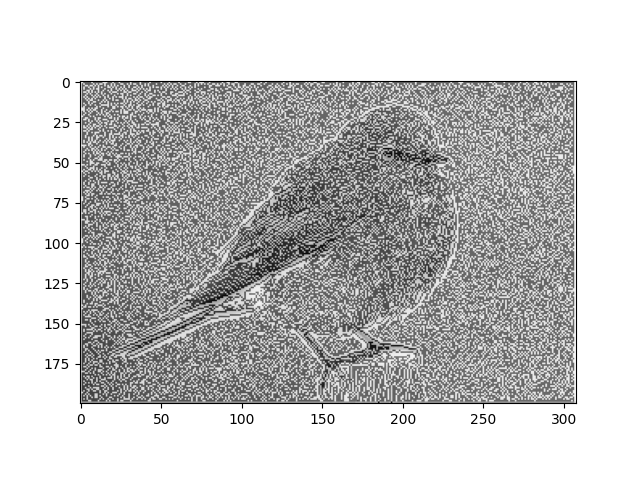
\includegraphics{Cost_Bird_Modified.png}
	\caption{\label{fig:bird_cost_mod}Cost matrix of blue bird using modified Z-crossing score}
\end{figure}
In figure \ref{fig:bird_cost_ori}, there is thin one pixel white edge (zero cost) around the bird. In theory, this would be an excellent cost matrix since the edge surrounding the bird is so sharp and precise. However, since the edge is only one pixel in width, the edge cannot be adjacent/orthogonal neighbors with itself along diagonals. To follow a diagonal, the edge may be diagonally connected with itself as seen in \ref{fig:bird_cost_mod_marked} (diagonal edge pixels marked red). Since diagonal pixels are not directly connected, the only way to get from one edge pixel to another diagonal to it is by traveling horizontally/vertically to a new pixel and then vertically/horizontally to the edge pixel. During this process, there may be other non-edge pixels that are close by that have a lower cost to travel to. Thus, the one pixel white edge will be derailed and led astray as seen in figure \ref{fig:bird_16}.

\begin{figure}[H]
	\centering
	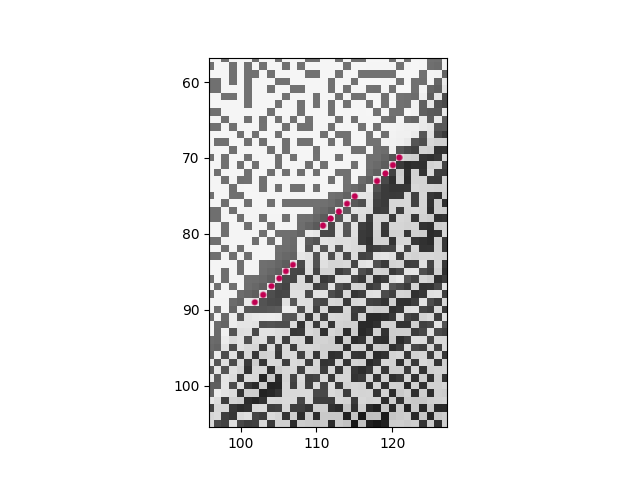
\includegraphics{cost_closeup_back_bird_marked.png}
	\caption{\label{fig:bird_cost_mod_marked}Zoomed in on cost matrix of blue bird's back using original Z-crossing score, parts of the one pixel white edge that are diagonal to each other are marked in red}
\end{figure}

The theory about is shown in practice in figure \ref{fig:bird_orient} and figure \ref{fig:gradient} where in both cases the scissors work much better cutting horizontally compared to cutting diagonally.

\begin{figure}[H]
\raisebox{-.5\height}{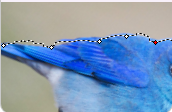
\includegraphics{bird_feather.png}}%
\hfill
\raisebox{-.5\height}{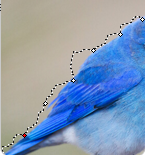
\includegraphics{bird_feather_2.png}}%
\caption{\label{fig:bird_orient} Original intelligent scissors on blue bird's back, one the left the back of the bird is rotated to horizontal position, while on the right bird is left in the original orientation.}
\end{figure}


\begin{figure}[H]
\raisebox{-.5\height}{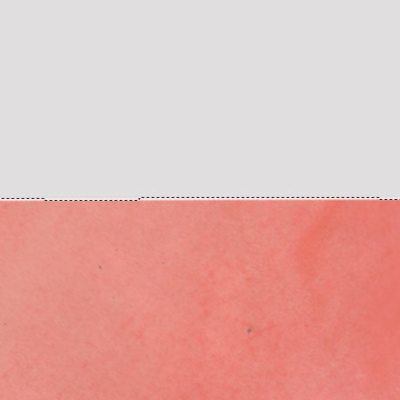
\includegraphics[scale = 0.75]{horizontal_flat2.png}}%
\hfill
\raisebox{-.5\height}{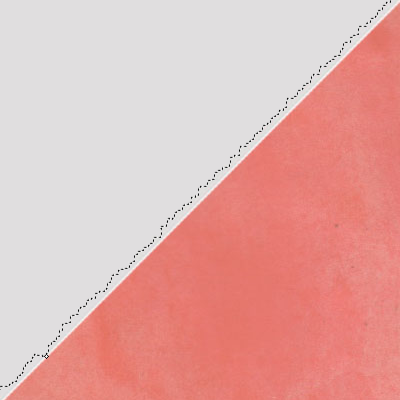
\includegraphics[scale = 0.75]{diagonal_jumps2.png}}%
\caption{\label{fig:gradient} Original intelligent scissors on grey/red plane. On the left the planes intersect horizontally, and on the right the planes intersect diagonally.}
\end{figure}


On the other hand, in figure \ref{fig:bird_cost_mod} (cost computed using modified Z-crossing score), there is a thin one pixel black edge (cost of one) around the bird. Closely surrounding the thin black edge is a much thicker white edge. The white edge closely follows the birds outline and is much more continuous than in figure \ref{fig:bird_cost_ori}. The increase in thickness of the white edge makes it much more robust to the noise inside and outside the bird. This robustness boosts the performance of the scissors by supporting continuous cuts that follow the outline of the bird as seen in figure \ref{fig:bird_4}.\\

At first glance, it seems like the inverted implementation of the Z-crossing score does it all. However, taking a closer look, it does not precisely follow the outline of the image. Instead, it "outlines the outline" of the image. However, more problems come into play when there is a plain background. Since the Z-crossing score is inverted, the plain background will have an extremely low cost (due to zero Z-crossing score) as seen in figure \ref{fig:shark_cost_mod}. This will misguide the scissor to cut around the background, rather than around the image as seen in figure \ref{fig:shark_cut_mod}.

\begin{figure}[H]
	\centering
	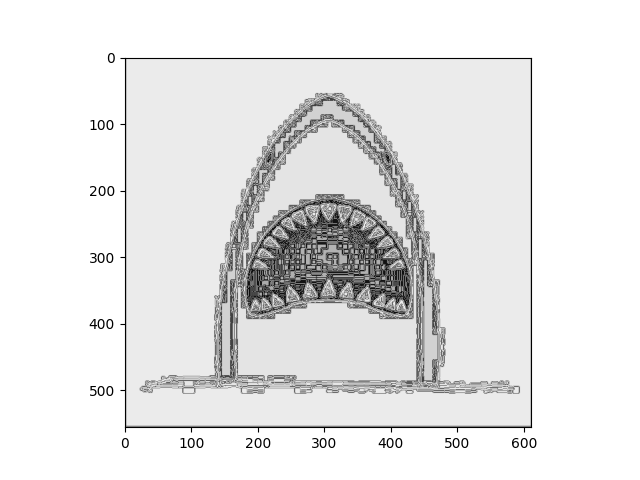
\includegraphics[scale = 0.5]{Cost_Shark_Modified.png}
	\caption{\label{fig:shark_cost_mod}Cost matrix of shark using modified Z-crossing score}
\end{figure}

\begin{figure}[H]
	\centering
	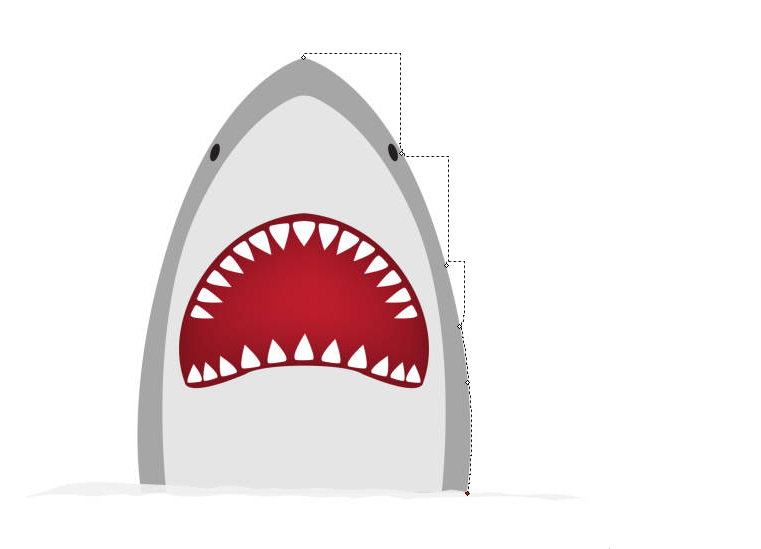
\includegraphics[scale = 0.5]{shark_modified_cut.png}
	\caption{\label{fig:shark_cut_mod} Cutting out shark using modified intelligent scissors}
\end{figure}

Now if we use the original implementation of the Z-crossing score, the cost of the plain background is much higher (due to Z-crossing score of one) as seen in figure \ref{fig:shark_cost_mod}. Thus, the original implementation is much better at tracing the shark as seen in figure \ref{fig:shark_cut_mod}.

\begin{figure}[H]
	\centering
	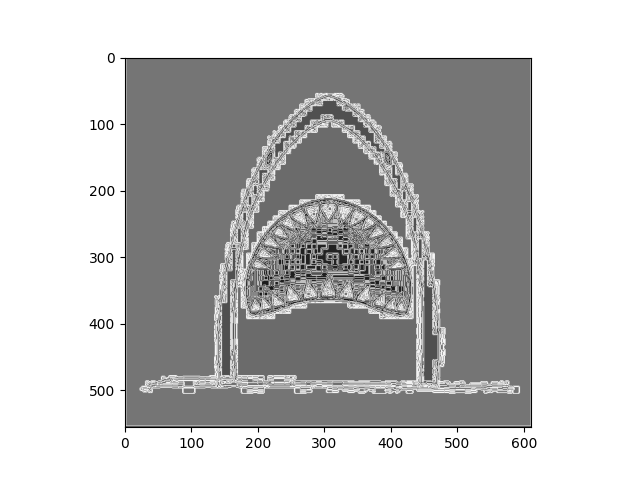
\includegraphics[scale = 0.5]{Cost_Shark_Original.png}
	\caption{\label{fig:shark_cost_mod}Cost matrix of shark using original Z-crossing score}
\end{figure}

\begin{figure}[H]
	\centering
	
\includegraphics[scale = 0.5]{shark_cut.png}
	\caption{\label{fig:shark_cut_mod} Cutting out shark using original intelligent scissors}
\end{figure}

We have seen that both implementations of intelligent scissors has its flaws. The original/correct implementation of intelligent scissors is extremely bad at handling curves in images due to the single pixel edge's inability of connecting directly with diagonal edge pixels. However, the reason the user wants to use intelligent scissors is because the object being cut out is not a horizontal/vertical cut, but rather has many curves that makes hand cutting it tedious. As a result, the current implementation of edge weights is not good enough. It could be a good idea to consider diagonal pixels as neighbors that are directly connected. This would increase the scissor's ability to handle curves.\\

In the meantime, the modified intelligent scissor with the inverse Z-cross scoring appears to handle curves much better. However in some cases where the background is very plain, the scissors will fail spectacularly. Despite these risks, this modified intelligent scissor works fairly well for most images I tested.\\

A weakness that appears in both implementation is their ability to handle shadows and highlights in images. The intelligent scissors tend to follow the highlights/shadows rather than the actual object.

\section{Naive vs. Optimized Dijkstra's}

To test the speedup of optimized vs naive Dijkstra, I randomly selected a starting vertex and ran Dijkstra till all shortest paths were found. The speedup in practice is does not match up with the improvement of $O(|V|^2)$ versus $O((|V|+|E|)\log|V|)$ as seen in table \ref{table:wrong_complexity}.

\begin{table}[H]
\begin{tabular}{|l|l|l|l|l|l|}
\hline
Image & Optimized (s) & Naive (s) & In Practice (xFaster) & In Theory (xFaster) & Total Vertices \\ \hline
sample & 0.292 &  6.172 & 21.108 &  1294.098 & 61600\\ \hline
french bulldog & 1.114 &   45.898 & 41.175 &  4482.332 & 240000\\ \hline
bear cub & 0.208 &   4.383 & 21.006 & 1077.281 & 50325\\ \hline
sleeping fox & 1.219 &   63.107 & 51.727 &  4756.210 & 256000\\ \hline
deer & 21.201 &  1729.717 &  81.583 &  41706.655 & 2670000\\ \hline
\end{tabular}
\caption{\label{table:wrong_complexity} Comparing in-practice speed up to theoretical speedup assuming a theoretical improvement of $O(|V|^2)$ versus $O((|V|+|E|)\log|V|)$.}
\end{table}


The reason is because the $O(|V|^2)$ time complexity is the worst case scenario, where each vertex is connected to all the other vertices. Only in this case, will it take approximately $O(|V|$) operations to find the minimum cost vertex. In our situation, each vertex is only connected to neighboring vertices adjacent/orthogonal to it. Thus, the number of vertices in \textbf{todo} is approximately equal to the number of vertices that border the pixels that have been locked-in. In figure \ref{fig:visited_show}, all the vertices that have been visited are darkened, and the pixels that lie on the very edge of the darkened area represent pixels currently in \textbf{todo}. Figure \ref{fig:todo_show} shows all the vertices currently in \textbf{todo} in red.

\begin{figure}[H]
	\centering
	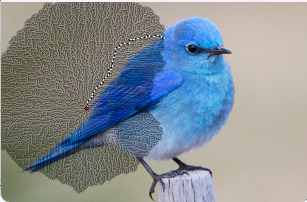
\includegraphics{show_visited.png}
	\caption{\label{fig:visited_show} Darkened pixels represent pixels that have been visited by Dijkstra's. The pixels that lie on the very edge of the darkened area are the pixels currently in \textbf{todo}}
\end{figure}

\begin{figure}[H]
	\centering
	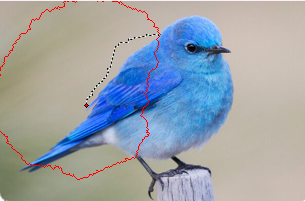
\includegraphics{todo_vis.png}
	\caption{\label{fig:todo_show} The red border are the pixels currently in \textbf{todo}}
\end{figure}

Since the largest border possible in our scenario is essentially the image parameter, a much better estimate of worse-case scenario time complexity is $O(V*(2*W+2*H))$ where $W=$ width of image in pixels and $H=$ height of image in pixels. The improvement of $O(V*(2*W+2*H))$ versus $O((|V|+|E|)\log|V|)$ matches up fairly well to the speedup obtained in practice as seen in the table \ref{table:right_complexity}. The reason they do not match up exactly is likely due to CPU spikes from other applications running on the computer. Furthermore, the time complexities calculated are approximate, and may be off by some coefficient or constant.

\begin{table}[H]
\begin{tabular}{|l|l|l|l|l|l|}
\hline
Image & Optimized (s) & Naive (s) & In Practice (xFaster) & In Theory (xFaster) & Total Vertices \\ \hline
sample & 0.252 &  5.163 & 20.472 & 21.344 & 61600\\ \hline
french bulldog & 1.154 &   44.387 & 38.453 &  37.352 & 240000\\ \hline
bear cub & 0.235 &   5.126 & 21.762 & 19.608 & 50325\\ \hline
sleeping fox & 1.298 &   57.961 & 44.631 &  38.644 & 256000\\ \hline
cute animal & 3.603 &  179.078 & 49.696 &  56.199 & 647513\\ \hline
cute puppy & 1.343 &  57.533 &  42.808 & 38.694 & 261042\\ \hline
\end{tabular}
\caption{\label{table:right_complexity} Comparing in-practice speed up to theoretical speedup assuming a theoretical improvement of $O(V*(2*W+2*H))$ versus $O((|V|+|E|)\log|V|)$.}
\end{table}

\section{Miscellaneous}
Another optimization took place in the image\_to\_graph function definition. I realized for large images, calculating the graph representation of the image took a very long time. I optimized this by calculating the horizontal and vertical edge weights outside the for-loop using matrix operations. And inside the forloop, each pixel only looks at the pixel to the right and the pixel beneath it, rather than all four neighbors. This minimizes the repetitiveness of examining the same edge weights multiple times.


\begin{figure}[H]
	\centering
	\includegraphics[scale=0.8]{deer_cut.png}
	\caption{\label{fig:visited_show} Thanks for reading!}
\end{figure}

\end{document}